% ============================================
% IV. THE NOVEL HIGH-THROUGHPUT COMPONENTS
% ============================================
\section{The Novel High-Throughput Components}
\label{sec:components}

We introduce two components for high-throughput parallel processing: the \textbf{Asynchronous Multi-Wallet Strategy} and the \textbf{Symbol-Sharded Lock-Free Model}. Together, these address blockchain-level nonce bottlenecks and server-side contention by adapting HFT lock-free concurrency patterns to blockchain's nonce constraints.

\subsection{Asynchronous Multi-Wallet Strategy}

Ethereum's sequential nonce requirement forces all transactions from a single wallet into strict serial order~\cite{wood2014yellowpaper}. Our strategy creates a one-to-one mapping between trading symbols and dedicated wallets, enabling independent transaction lanes. Trades for different symbols use separate nonce sequences, breaking the single-wallet bottleneck, as the results in Section~\ref{sec:results} demonstrate.

\subsection{Symbol-Sharded Lock-Free Model}

Multi-wallet solves the on-chain bottleneck, but Architecture~4 showed it shifts contention to the server (latency increased from 2.9s to 27.2s). The Symbol-Sharded Lock-Free Model extends symbol-based parallelism to internal data structures using dedicated, lock-free concurrent queues per symbol:

\begin{enumerate}
    \item \textbf{Routing:} Incoming trades route immediately to symbol-specific queues.
    \item \textbf{Parallel Consumption:} Dedicated worker threads consume from each symbol's queue.
    \item \textbf{Lock-Free Processing:} .NET's \texttt{ConcurrentQueue<T>} (Michael-Scott algorithm~\cite{michael1996lockfree}) uses CAS operations instead of locks, ensuring non-blocking, thread-safe operations.
    \item \textbf{Dedicated Submission:} Each worker uses its symbol's dedicated wallet for blockchain submission.
\end{enumerate}

This end-to-end symbol-sharded architecture eliminates server-side contention, reducing latency by 44\% (27.2s$\rightarrow$15.4s). Combined, these components achieve 31.19~tx/sec (\textbf{2.8$\times$} over conventional designs), ensuring the submission layer sustains rates exceeding blockchain capacity (\textbf{contribution C1}).

\begin{figure}[!ht]
    \centering
    \begin{subfigure}[b]{0.38\textwidth}
        \centering
        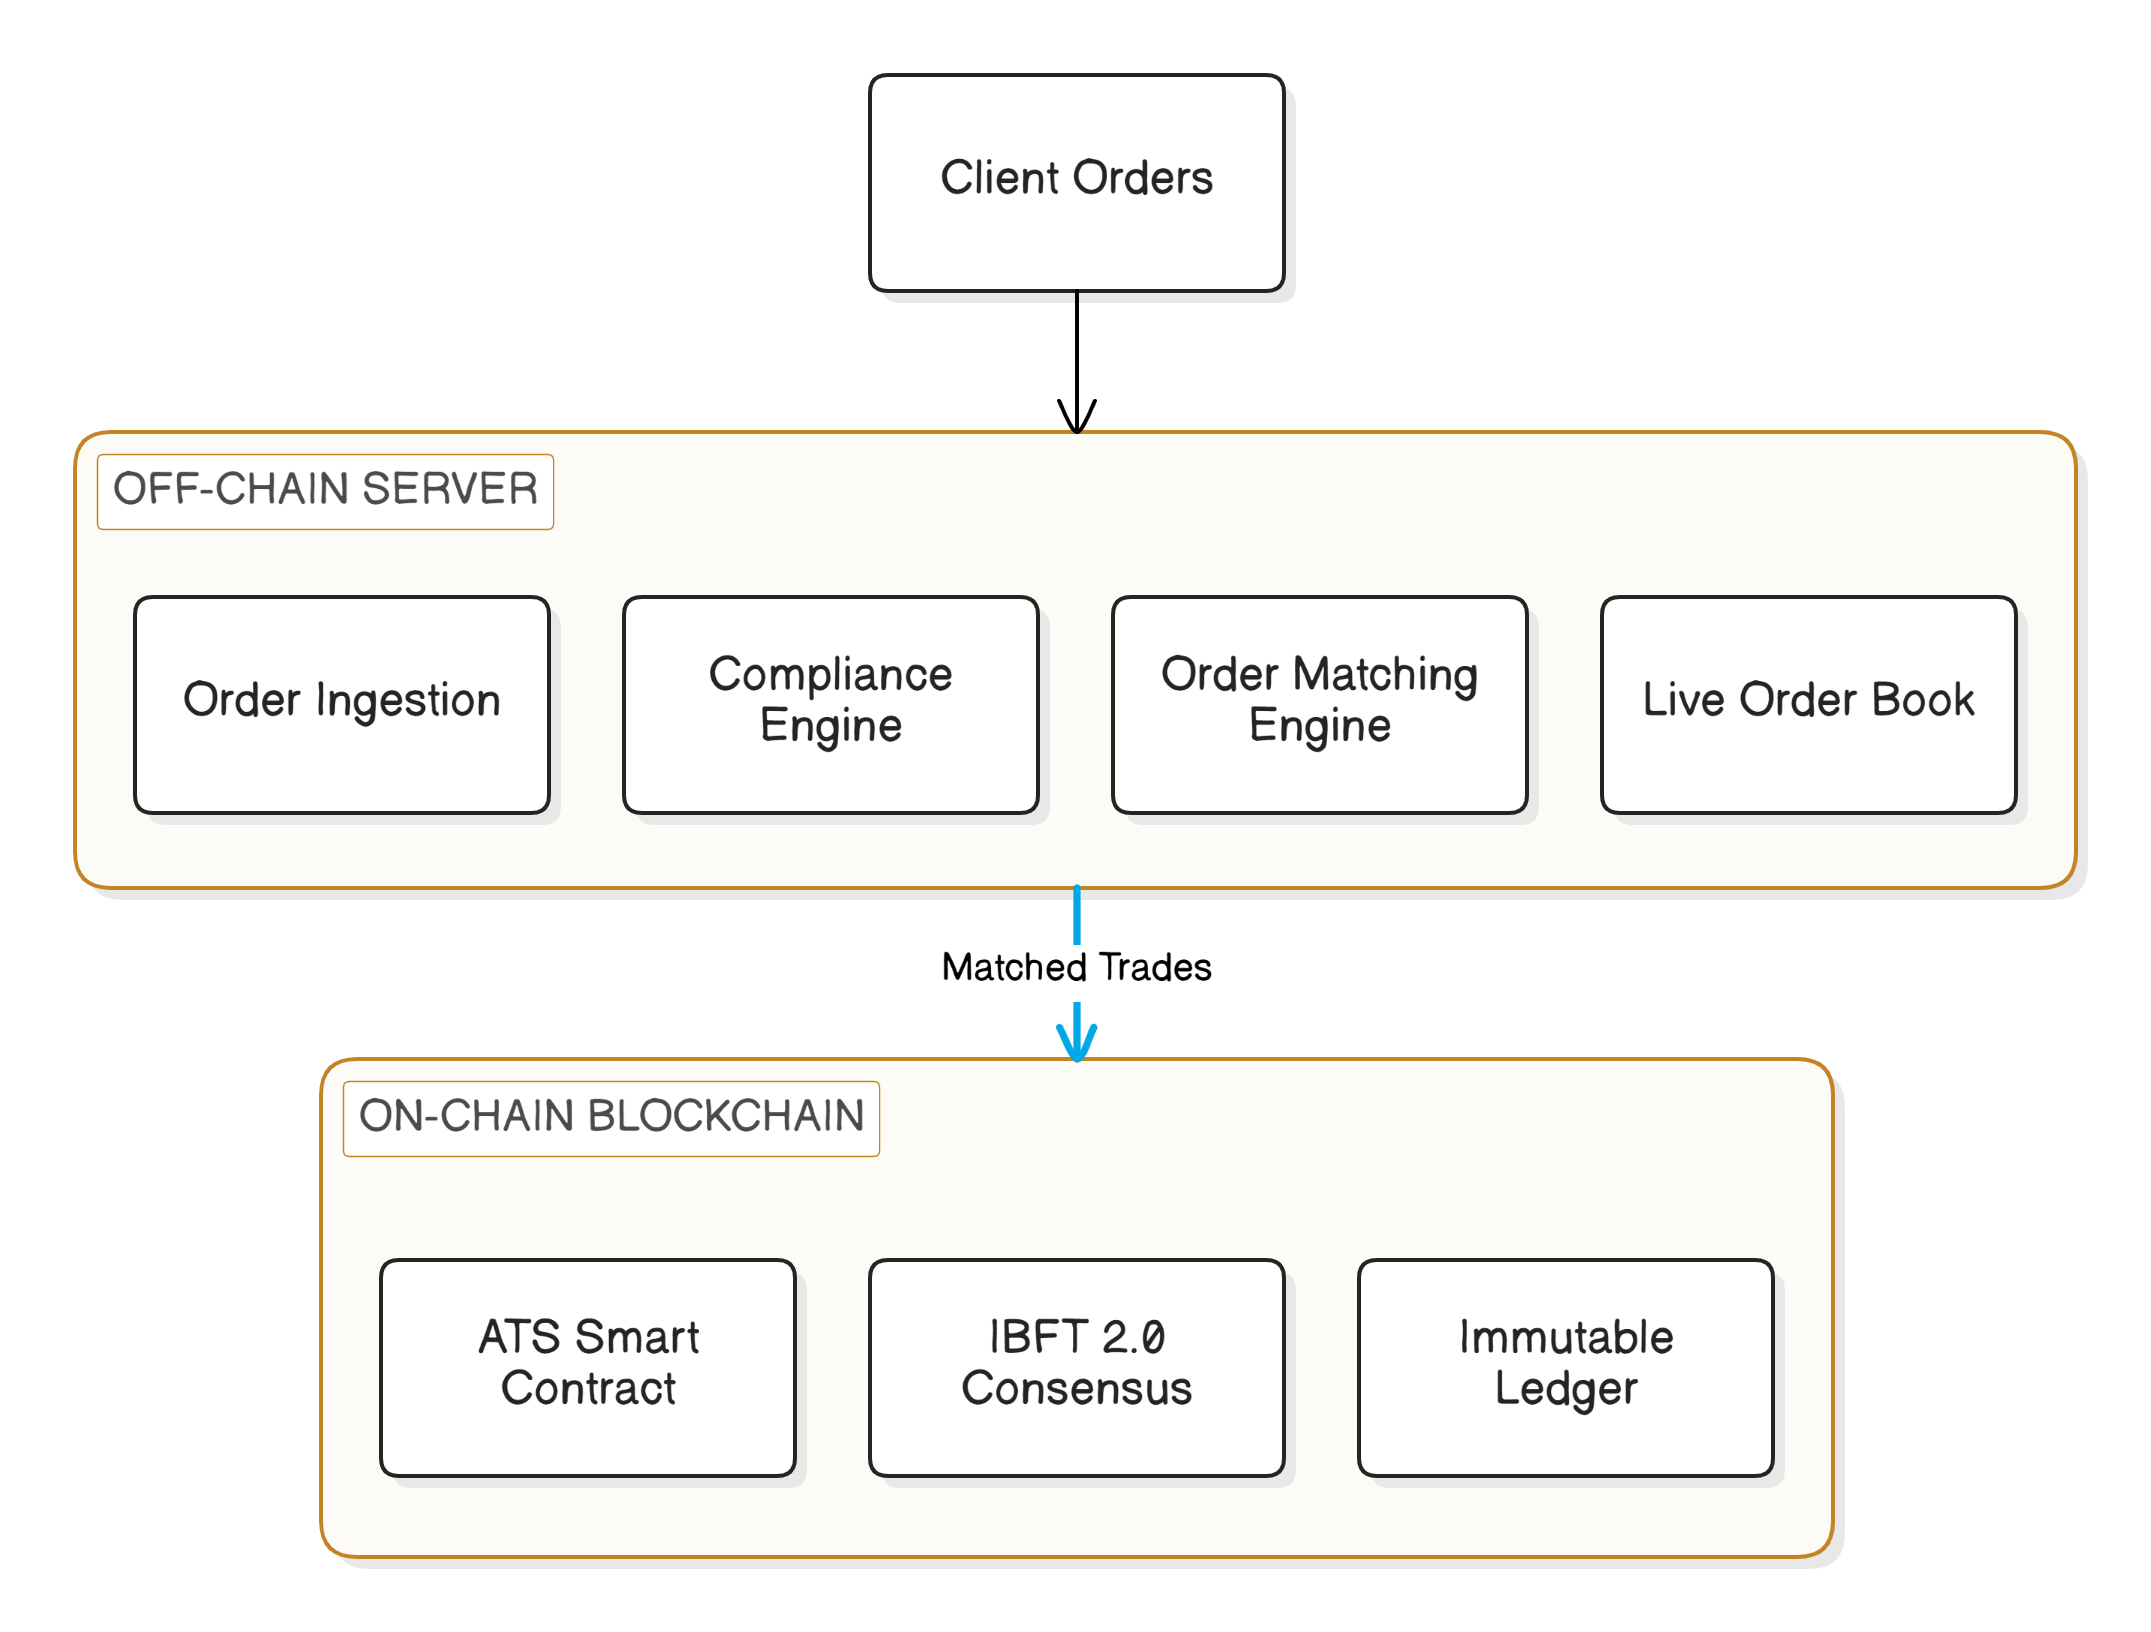
\includegraphics[width=\textwidth]{images/two-layer-model.png}
        \caption{Two-Layer Hybrid Architecture}
        \label{fig:two_layer_model}
    \end{subfigure}
    \hfill
    \begin{subfigure}[b]{0.38\textwidth}
        \centering
        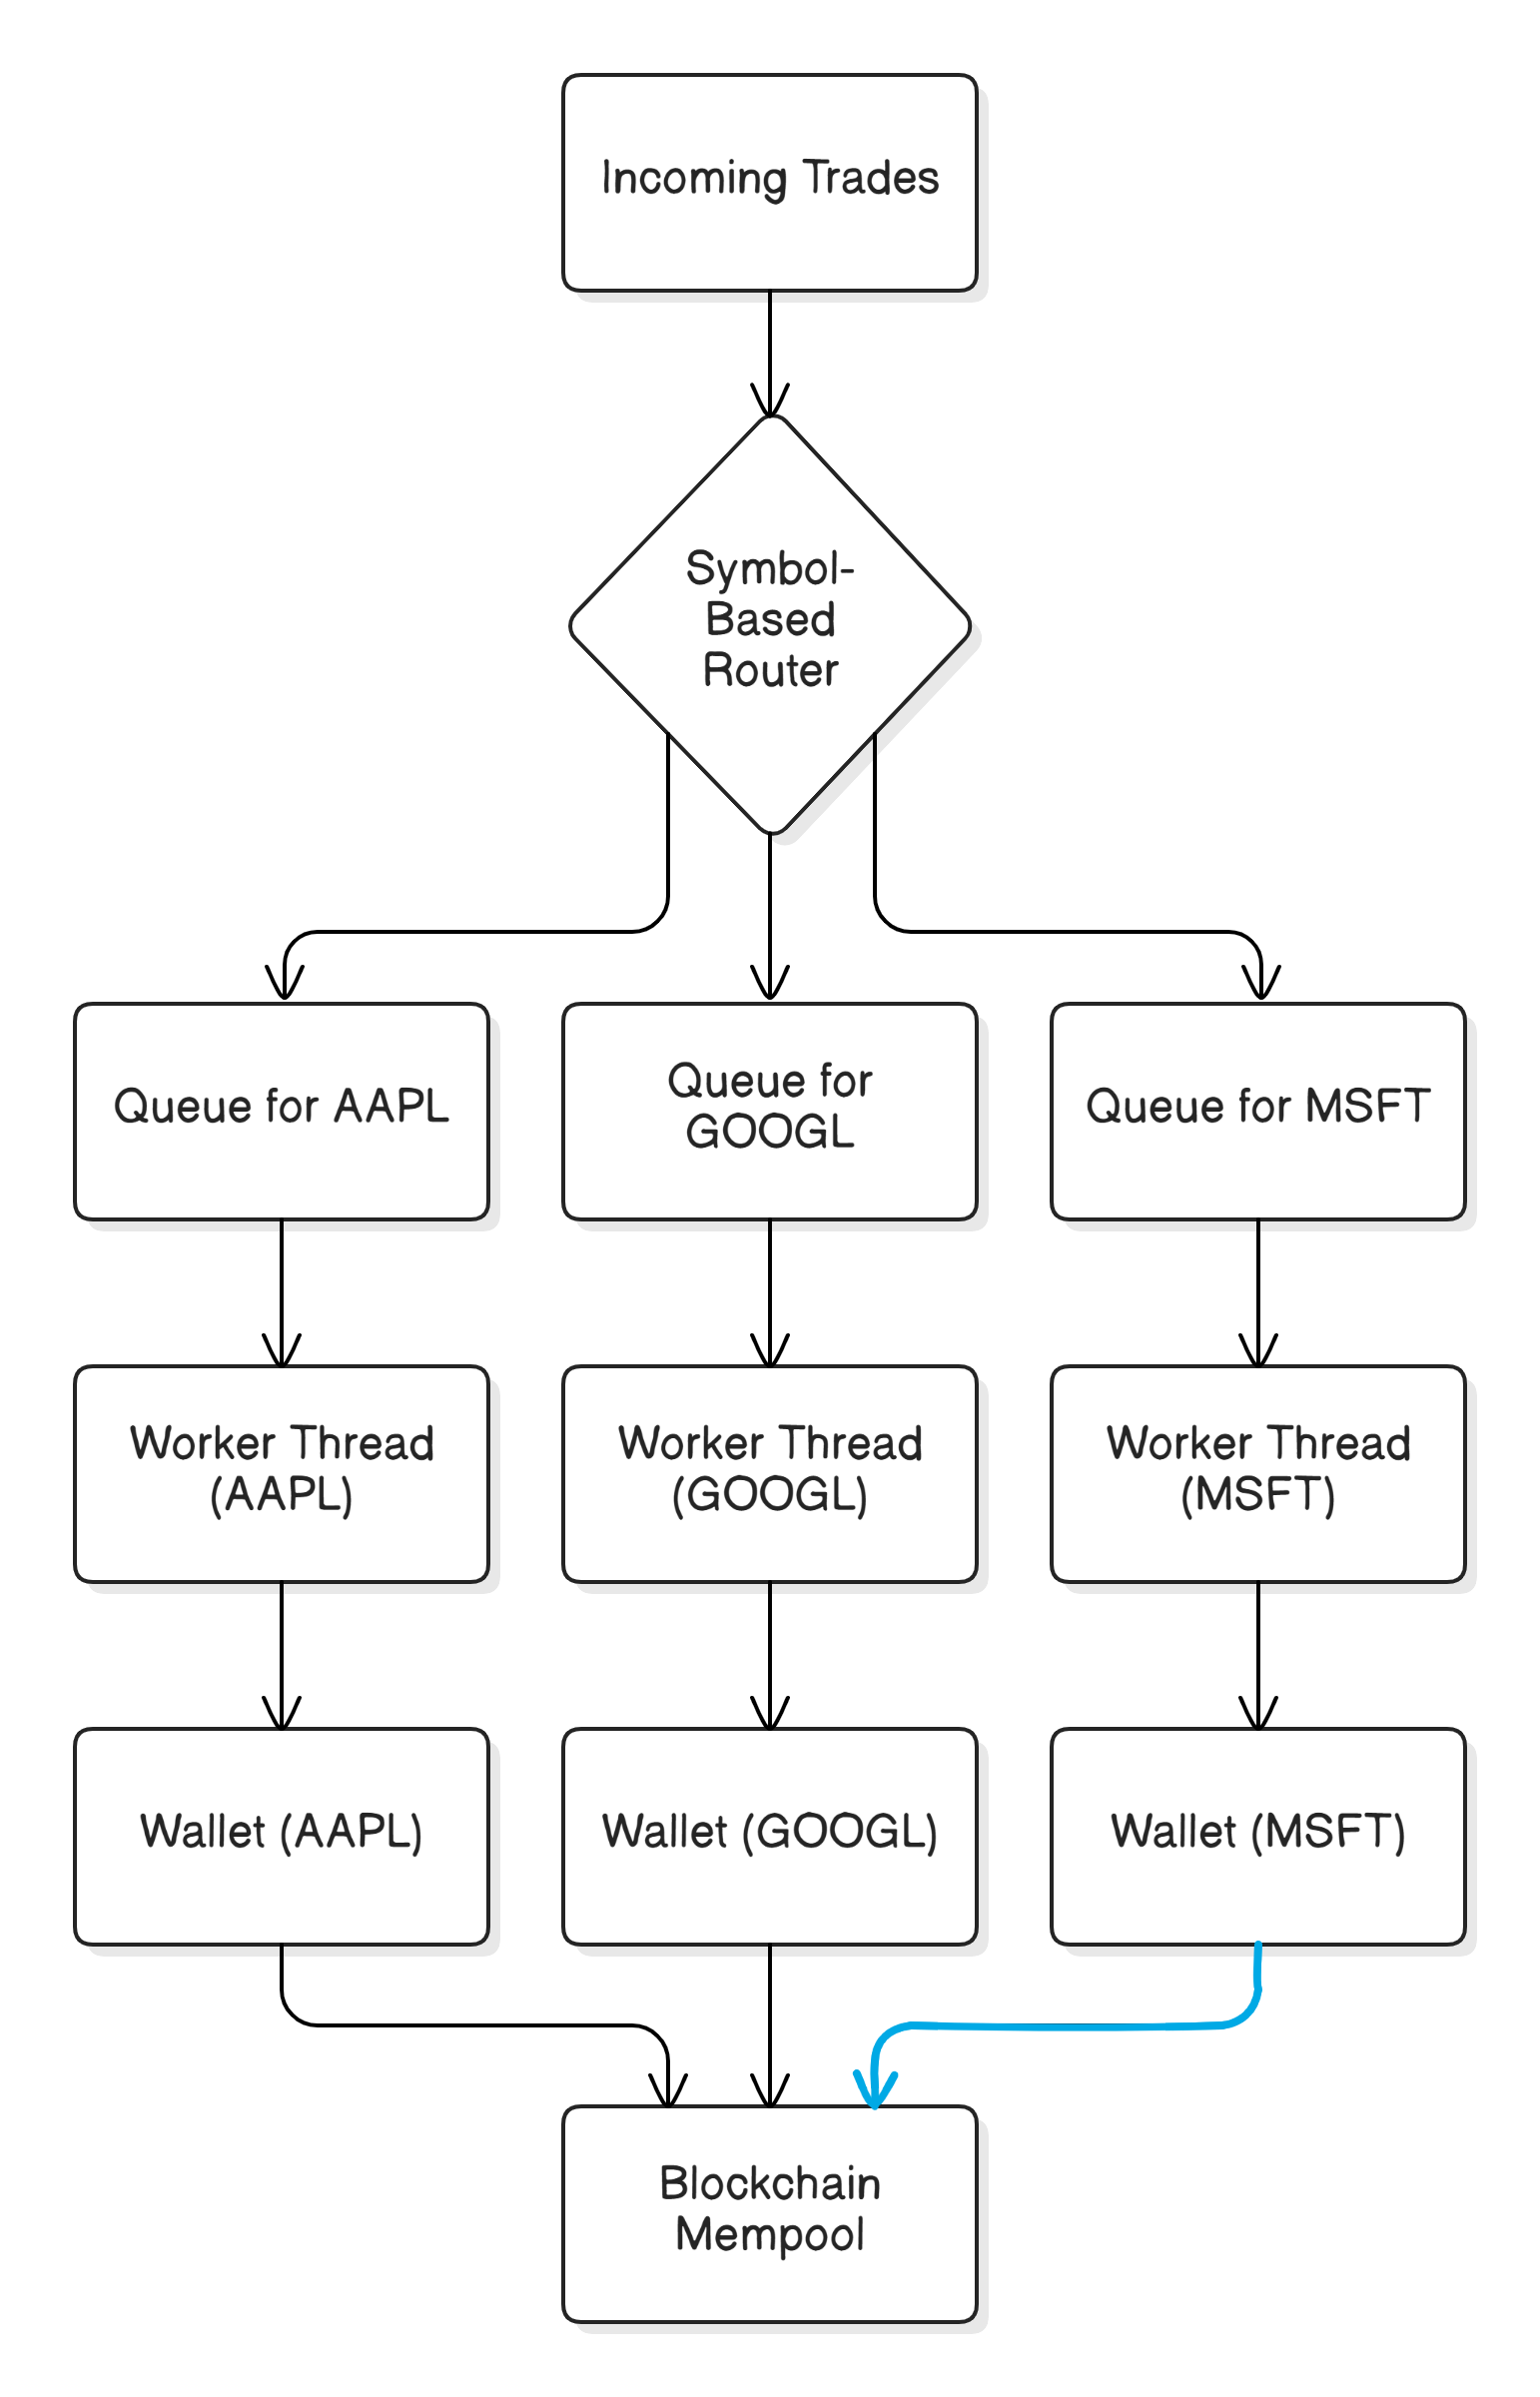
\includegraphics[width=\textwidth]{images/symbol-sharded-lock-free-model.png}
        \caption{Symbol-Sharded Lock-Free Model}
        \label{fig:symbol_sharded_model}
    \end{subfigure}
    \caption{System architecture: (a) Two-layer model separating off-chain compliance from on-chain settlement, (b) Symbol-sharded lock-free model showing end-to-end alignment from symbol queues to dedicated wallets. In both diagrams, rectangles denote processing components and arrows indicate data flow direction; the diamond in~(b) denotes the symbol-based routing decision.}
    \label{fig:architecture}
\end{figure}
